\documentclass[12pt]{ctexart}
\usepackage{geometry}       % 设置页面整体布局
\geometry{top=2.5cm, bottom=2.5cm, left=2cm, right=2cm}
\usepackage{fancyhdr}       % 设置页眉页脚布局
\pagestyle{fancy}
\rhead{\thepage}            % 设置右页眉为页数
\chead{中国科学技术大学}
\cfoot{}                    % 设置中间页脚为空
\usepackage{amsmath}        % 数学公式宏包
\numberwithin{equation}{section}
\usepackage{esint}          % 交叉引用宏包
\usepackage[colorlinks,     % 设置引用的颜色
            linkcolor=black,
            anchorcolor=black,
            urlcolor=cyan,
            citecolor=black,
           ]{hyperref}
\usepackage{makecell}       % 插入表格宏包
\usepackage{longtable}      % 长表格宏包
\usepackage{appendix}       % 生成附录宏包
\usepackage{graphicx}       % 插入图片宏包
\usepackage{epstopdf}       % 插入eps图片宏包
\usepackage{cite}           % 文献引用宏包
\renewcommand{\thefigure}   % 设置图片编号格式
    {\thesection{}.\arabic{figure}}
\renewcommand{\thefootnote}{} % 设置角标编号不出现在文中
                            % 以\footnotetext{Footnotetext without footnote mark}使用
\usepackage{unicode-math}
\usepackage{listings}
\usepackage{hyperref}



\CTEXsetup[format={\Large\bfseries}]{section}

\begin{document}

\nocite{*}

\begin{center}
    \heiti \fontsize{24pt}{0}{旋光物质化学反应反应动力学研究\\——蔗糖转化反应}

    \vspace{12pt}

    \kaishu \fontsize{13.75pt}{0}禤科材
    

    \footnotetext{\textbf{实验日期:}2022年9月30日}
    \footnotetext{\textbf{作者简介:}禤科材(2002-),男,学号PB20030874,中国科学技术大学本科在读,专业方向为化学物理}
    \footnotetext{\textbf{联系方式:}电话 18108064415 ,邮箱 \href{mailto:ustcxkc@mail.ustc.edu.cn}{ustcxkc@mail.ustc.edu.cn}}

    \vspace{5pt}

    \songti \fontsize{12pt}{0}(中国科学技术大学化学与材料科学学院,安徽 合肥 230026)
\end{center}

\noindent\textbf{摘~~~\!要}~~~\!
在催化剂H$^+$浓度固定、水分子大量存在的情况下,蔗糖的水解为准一级
反应,其浓度与时间具有明确的关系。同时蔗糖具有旋光性,其水溶液的
旋光度与其浓度也具有明确的关系。本实验通过测定不同时间蔗糖水解
体系的旋光度,代入反应的动力学方程进行线性以及非线性拟合,可以得到反应的速率常数
$k$。根据不同温度下的反应速率常数,可以计算蔗糖水解的表观活化能。通过数理统计方法的合理运用,能够推测蔗糖水解副反应的机理为一级反应。
\newline
\textbf{关键字}~~~\!
{\kaishu 准一级反应;旋光度;反应速率常数;表观活化能}

\begin{center}
    {\LARGE\rmfamily\textbf{The Kinetic Study on Reaction of Sucrose Conversion}}

    \vspace{12pt}

    {\slshape Xuan Kecai}

    \vspace{5pt}

    (School of Chemistry and Material Science, USTC, Hefei 230026, China)
\end{center}

\noindent\textbf{Abstract}~~~\!
When the H$^+$ concentration of catalyst is fixed and a large
number of water molecules exist, the hydrolysis of sucrose is
a quasi first-order reaction, and its concentration has a
clear relationship with time. At the same time, sucrose has
optical rotation, and the optical rotation of its aqueous
solution has a clear relationship with its concentration. In
this experiment, the reaction rate constant $k$ can be
obtained by measuring the optical rotation of sucrose
hydrolysis system at different times and fitting it with both linear and nonlinear models. According to the reaction
rate constants at different temperatures, the apparent
activation energy of sucrose hydrolysis can be calculated.With the application of mathematical statistics, the mechanism of the side reaction of sucrose hydrolysis can be inferred as the first order reaction.
\newline
\textbf{Keywords}~~~\!
pseudo first order reaction; optical rotation;
reaction rate constant; apparent activation energy

\section{序言}

蔗糖,是食糖的主要成分,是双糖的一种,由一分子葡萄糖的半缩醛羟基
与一分子果糖的半缩醛羟基彼此缩合脱水而成。蔗糖有甜味,无气味,易
溶于水和甘油,微溶于醇。有旋光性,但无变旋光作用。蔗糖几乎普遍存在
于植物界的叶、花、茎、种子及果实中。在甘蔗、甜菜及槭树汁中含量尤为
丰富。蔗糖味甜,是重要的食品和甜味调味品。分为白砂糖、赤砂糖、
绵白糖、冰糖、粗糖。

多糖在酸性条件下可以水解,完全水解后生成单糖。在工业生产中,人们利用
多糖的水解制取葡萄糖;在生物体内,也时刻发生着多糖的催化水解反应。
因此,多糖水解反应动力学的研究有着重大意义。

\section{实验}
\subsection{实验原理}

酸性条件下,蔗糖可以水解成葡萄糖和果糖

\begin{align}
    \mathop{\mathrm{C_{12} H_{22} O_{11}}}_{\text{蔗糖}}
    + \mathrm{H_2 O}
    ~\mathop{\longrightarrow}^{\mathrm{H^+}}~
    \mathop{\mathrm{C_6 H_{12} O_6}}_{\text{葡萄糖}}
    + \mathop{\mathrm{C_6 H_{12} O_6}}_{\text{果糖}}.
\end{align}

由于反应物蔗糖呈右旋性($[\alpha]^{20}_{D}$ = 66.6$^\circ$),
生成物果糖的左旋性($[\alpha]^{20}_{D}$ = -91.9$^\circ$)大于
葡萄糖的右旋性($[\alpha]^{20}_{D}$ = 52.5$^\circ$),随着反应的
进行,体系的旋光度会不断减小。当其他条件固定时,旋光度$\alpha$与
反应物浓度$c$呈线性关系,体系最初的旋光度和蔗糖完全水解以后最终
体系的旋光度分别为
\begin{align}
    \alpha_0 = K_{\text{反应物}}c_{A}^0,
    \qquad
    \alpha_\infty = K_{\text{生成物}}c_{A}^0.
\end{align}

设当时间为$t$时,蔗糖浓度为$c_A$,则此时的旋光度为
\begin{align}
    \alpha_t = K_{\text{反应物}}c_{A} + K_{\text{生成物}}
    (c_A^0 - c_A).
\end{align}

由式(1.2)和式(1.3)可以计算出蔗糖的浓度为
\begin{align}
    c_A^0 &= \frac{\alpha_0 - \alpha_\infty}
        {K_{\text{反应物}} - K_{\text{生成物}}}
    = K'(\alpha_0 - \alpha_\infty), \\
    c_A &= \frac{\alpha_t - \alpha_\infty}
        {K_{\text{反应物}} - K_{\text{生成物}}}
    = K'(\alpha_t - \alpha_\infty).
\end{align}

当有大量水存在时,蔗糖的水解反应为准一级反应,满足积分式
\begin{align}
    \ln c_A = - kt + \ln c_A^0.
\end{align}

将式(2.4)和式(2.5)带入式(2.6),得
\begin{align}
    \ln (\alpha_t - \alpha_\infty)
        = - kt + \ln (\alpha_0 - \alpha_\infty).
\end{align}

通过$\ln(\alpha_t - \alpha_\infty) \sim t$图像的斜率可以求出
反应速率常数$k$;通过 Arrhenius 公式,可由不同温度下的速率常数$k$
求出反应的表观活化能。

\subsection{试剂与仪器}

分析纯蔗糖溶液(国药集团化学试剂有限公司,40 g 蔗糖溶于400 mL 水中、
20 g 蔗糖溶于400 mL 水中)、HCl 溶液(国药集团化学试剂有限公司,
4 mol·dm−3 和2 mol·dm−3)。

MCP500 型旋光仪(Anton Paar(Shanghai)Trading Co., Ltd.)、
BT00-2J 型蠕动泵驱动器(Longer-Pump®)、HK-2A 型超级恒温水水浴
(南京南大万和科技有限公司)、150 mL 锥形瓶、25 mL 移液管、50 mL
移液管、100 mL 容量瓶、100 mL 量筒、500 mL 广口瓶。

\subsection{实验方法}
\subsubsection{蔗糖转化旋光度的测定}

将50.00 mL 已恒温的HCl 溶液注入到50.00 mL 已恒温的蔗糖溶液中,立即
开始计时。将混合的的反应物摇匀并装满已经预热到的样品管,放入旋光仪
内,每隔30 s 测量一次的旋光度。离开始起反应的3min 内开始记录,持续
记录35$\sim$40 min。

\subsubsection{\texorpdfstring{$\alpha_{\infty}$的测定}{反应完全进行时溶液旋光度的测定}}

将剩余的反应液放置于 60$^\circ$C 的水浴上温热 30 min,使其加速
反应至完全,然后冷却至原来温度,再测量此溶液的旋光度,记录不同温度、
反应浓度下的$\alpha_{\infty}$值。

\section{结果与讨论}
\subsection{\texorpdfstring{速率常数$k$和半衰期$t_{1/2}$}{速率常数和半衰期}}

实验共设置了 10 组平行实验,各组实验的反应条件和测量计算结果如表 1
所示。其中,对于组1和组2,测得两种条件下的$\alpha_{\infty}$分别为
-0.4525$^\circ$和0.4814$^\circ$,用 Mathematica 分别绘制
$\ln(\alpha_t-\alpha_{\infty}) \sim t$ 图如图 3.1 和图 3.2 所示。

\begin{figure}[!h]
\begin{minipage}[t]{0.5\linewidth}
    \centering
    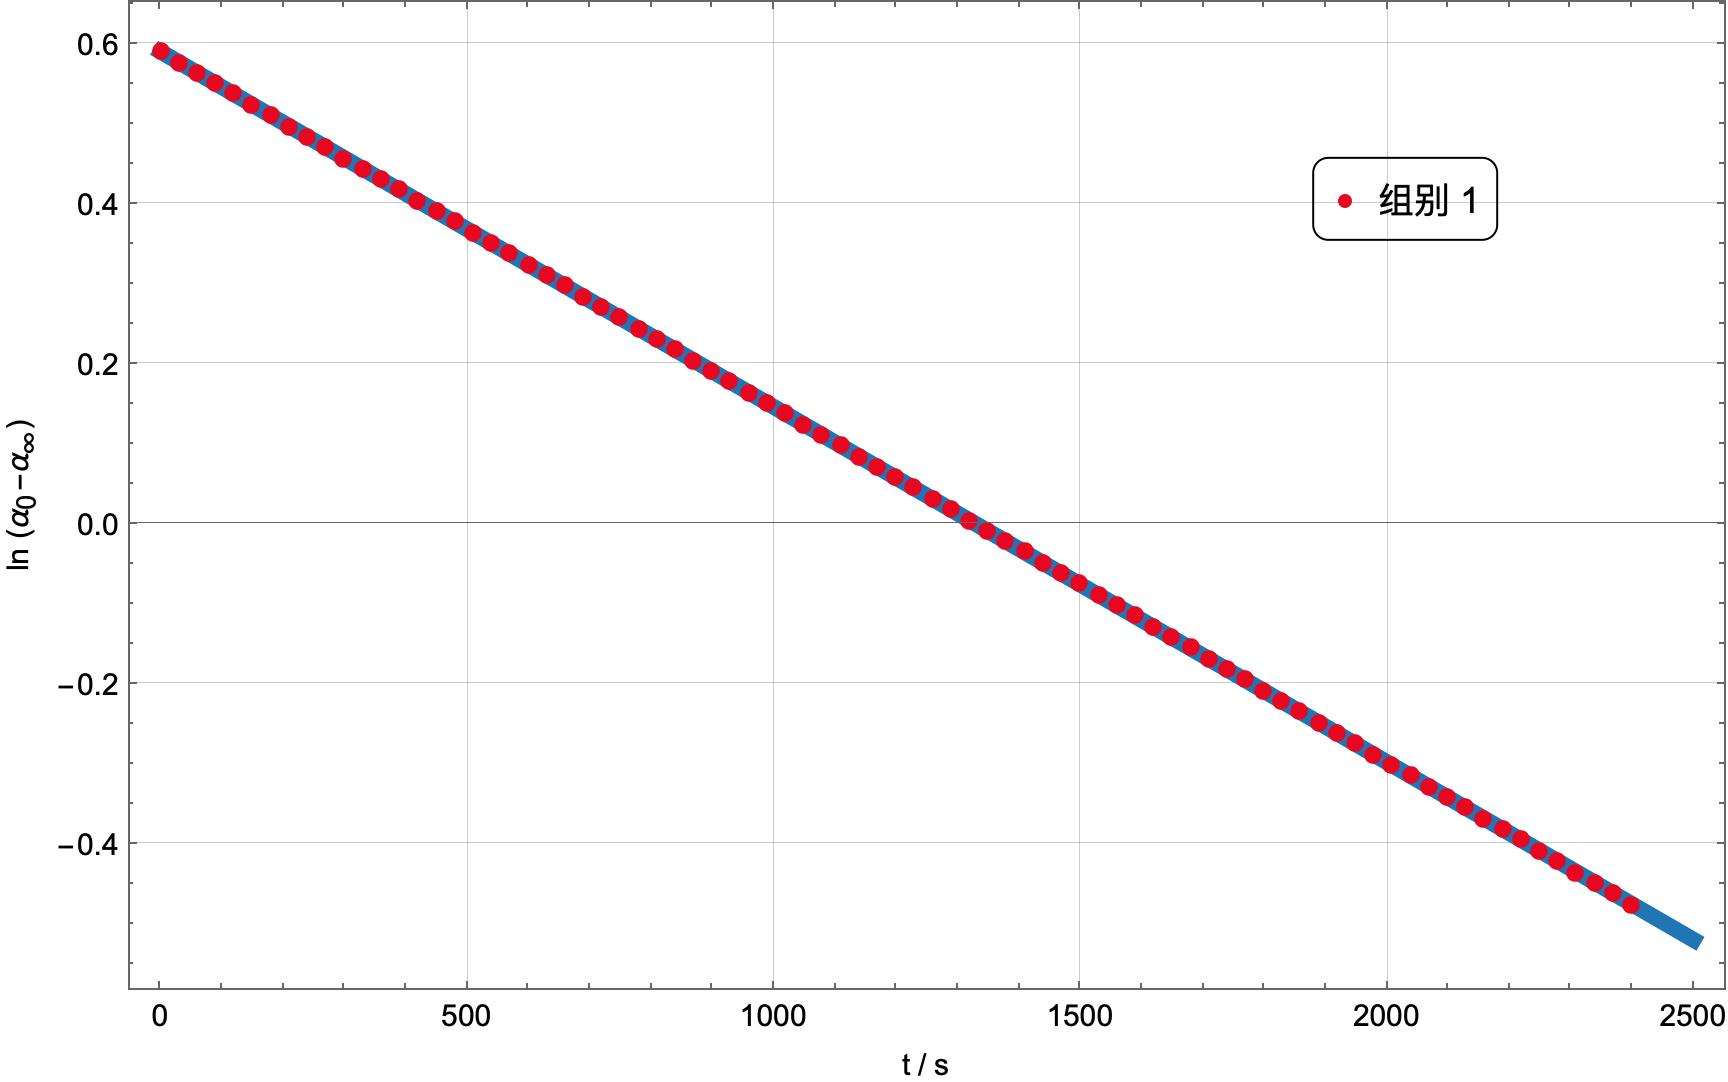
\includegraphics[scale=0.29]{first.jpg}
    \label{fig:first}
    \caption{组别 1 拟合图像}
\end{minipage}
\begin{minipage}[t]{0.5\linewidth}
    \centering
    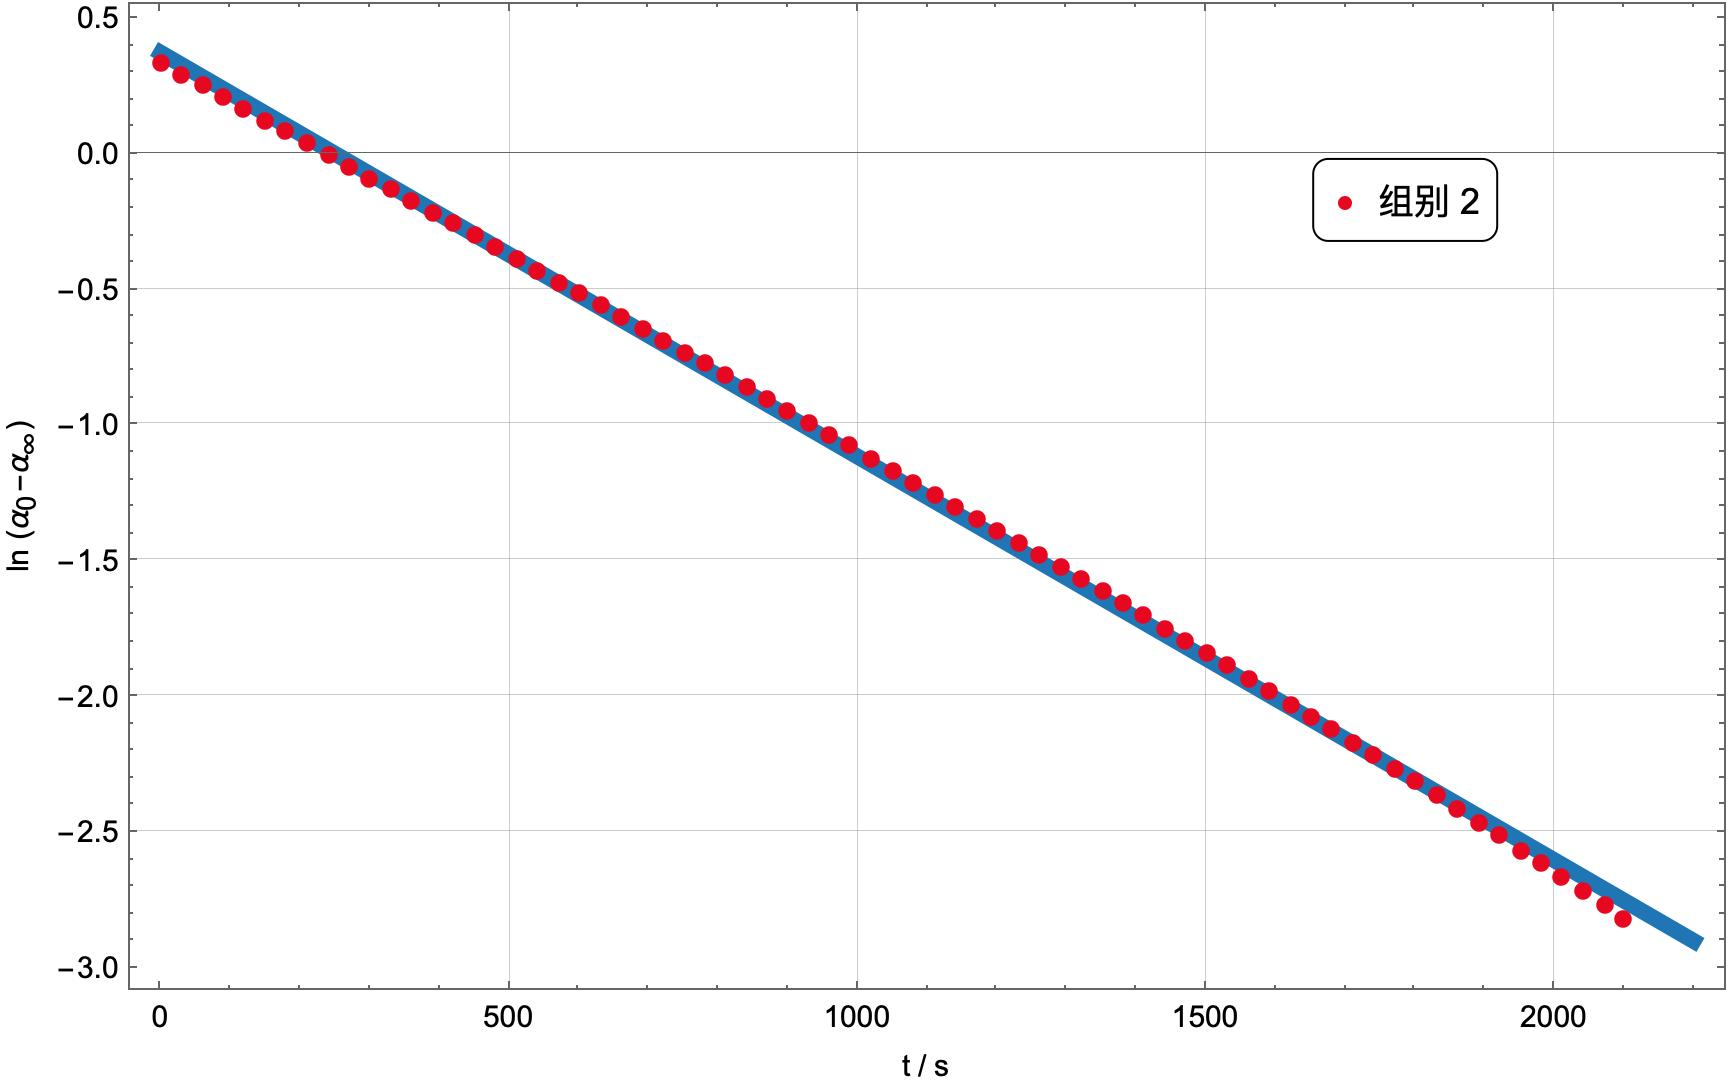
\includegraphics[scale=0.29]{second.jpg}
    \label{fig:second}
    \caption{组别 2 拟合图像}
\end{minipage}
\end{figure}

其中,组 1 拟合得到的曲线方程为$\ln(\alpha_t-\alpha_{\infty})$ =
-4.438$\times$10$^{−4}t$ + 0.5910,由式 (1.7) 得到该条件下的反应
速率常数$k_1$ = 4.438$\times$10$^{−4}$s$^{-1}$;组 2 拟合得到的
曲线方程为$\ln(\alpha_t-\alpha_{\infty})$ = -1.488$\times$
10$^{-3}t$ + 0.3713,反应速率常数$k_2$ = 1.488$\times$10$^{-3}$
s$^{-1}$。

用相同的方法计算 10 组实验的速率常数$k$,再根据准一级反应$t_{1/2}$
= $\ln 2/k$得到每一组反应的半衰期。10 组实验的
$\ln(\alpha_t-\alpha_{\infty}) \sim t$拟合图像如图 \ref*{fig:inone} 所示。

\begin{figure}[!h]
    \centering
    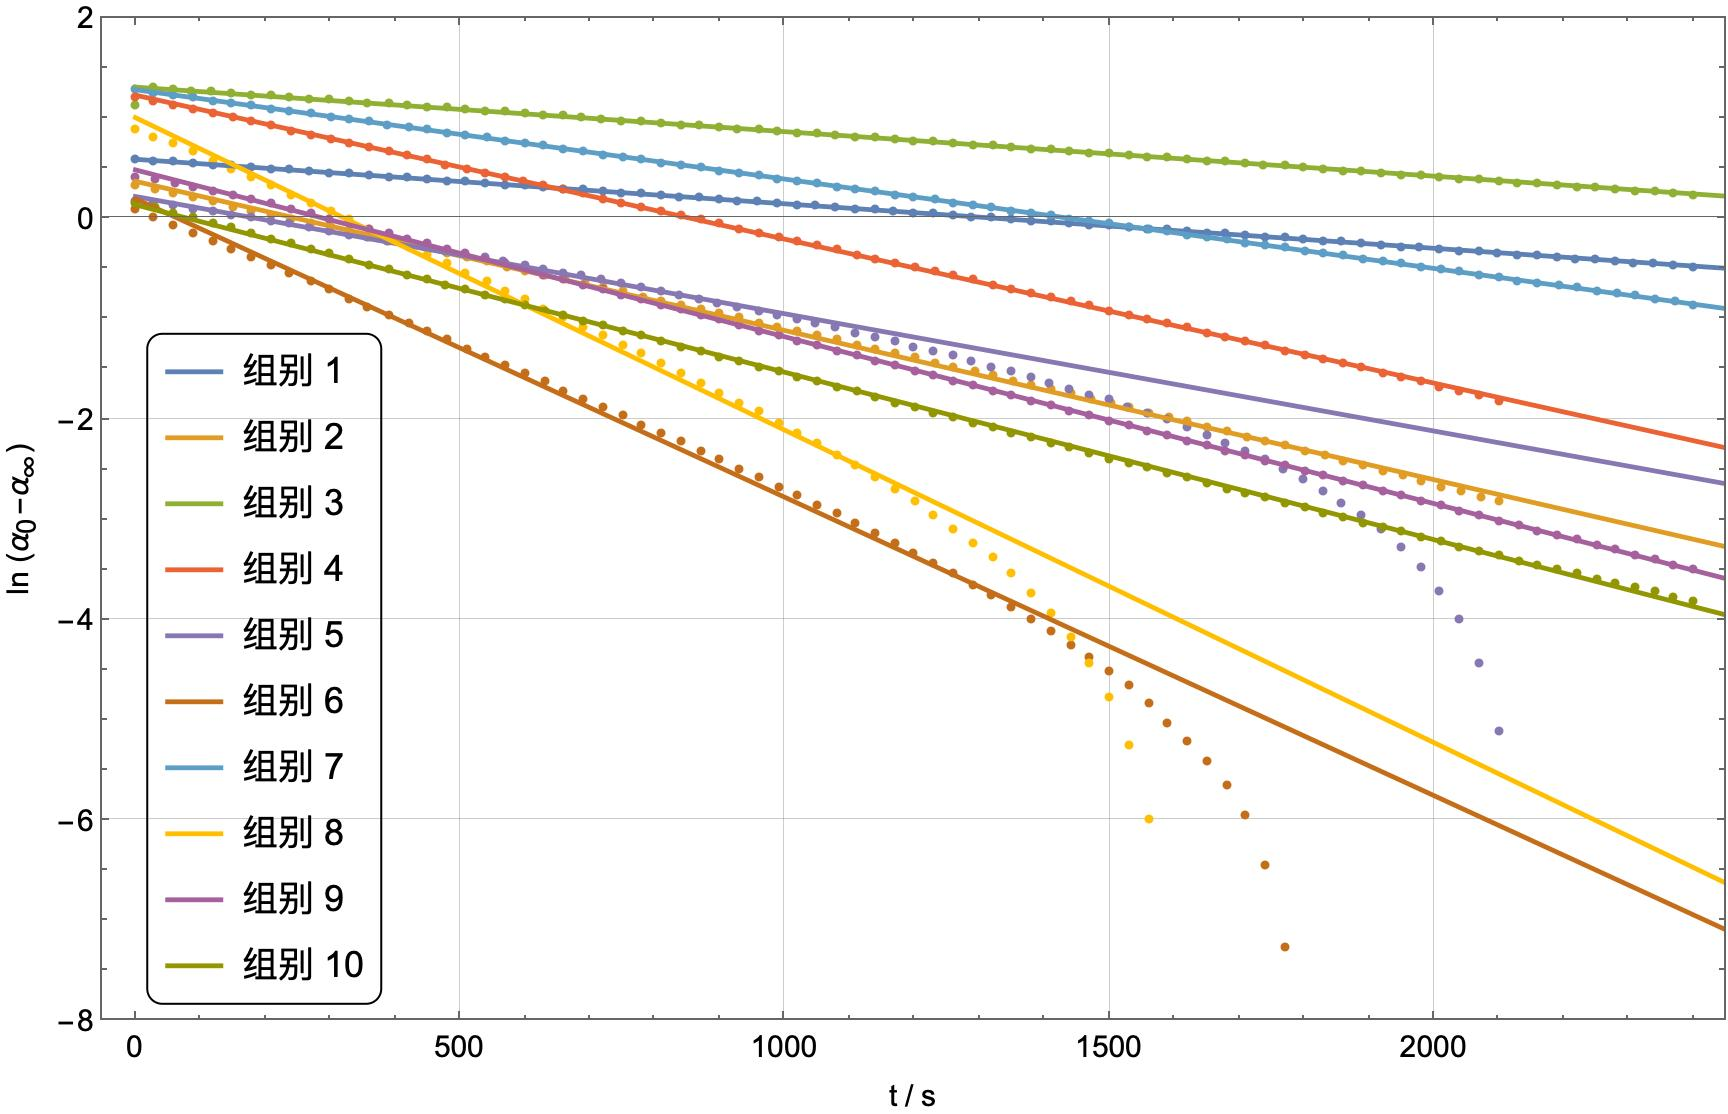
\includegraphics[scale=0.50]{inone.jpg}
    \label{fig:inone}
    \caption{各组实验数据拟合图像}
\end{figure}

\newpage
由于$t > 1200$s 时可以明显看出部分组的实验数据已偏离准一级反应,
故图 3.3 中组别 5、6、8 的拟合直线仅由$0 \le t \le 1200$s 的数据得到。

可以计算出 10 组实验的速率常数和半衰期如表 1 所示。

\begin{longtable}{|c|cccccccccc|}
    \caption{反应条件与测量结果} \\
    \hline
    组别 & 1 & 2 & 3 & 4 & 5 & 6 & 7 & 8 & 9 & 10\\
    \hline
    温度/$^\circ$C & 30.00 & 30.00 & 30.00 & 30.00 & 35.00 & 35.00 & 35.00 & 35.00 & 40.00 & 40.00 \\
    蔗糖浓度 & 低 & 低 & 高 & 高 & 低 & 低 & 高 & 高 & 低 & 低 \\
    盐酸浓度/mol$\cdot$L$^{-1}$ & 2 & 4 & 2 & 4 & 2 & 4 & 2 & 4 & 2 & 2 \\
    $k$/$\times 10^{-4}$s$^{-1}$ & 4.438 & 14.88 & 4.438 & 14.36 & 11.69 & 29.76 & 8.912 & 31.16 & 16.64 & 16.70 \\
    $t_{1/2}$/ min & 26.02 & 7.765 & 26.03 & 8.045 & 9.878 & 3.882 & 12.96 & 3.707 & 6.943 & 6.919 \\
    \hline
\end{longtable}

\subsection{\texorpdfstring{$\alpha_0$的计算}{溶液初始旋光度的计算}}

初始蔗糖溶液的旋光度$\alpha_0$值即为拟合曲线的截距值。 求解方程 $\ln(\alpha_{0} - \alpha _{\infty})= b_i$ 可以分别解得不同组别的初始旋光度,如表 2 所示。

\begin{longtable}{|c|ccccc|}
    \caption{初始旋光度} \\
    \hline
    组别 & 1 & 2 & 3 & 4 & 5\\
    \hline
    温度/$^\circ$C & 30.00 & 30.00 & 30.00 & 30.00 & 35.00  \\
    蔗糖浓度 & 低 & 低 & 高 & 高 & 低 \\
    盐酸浓度/mol$\cdot$L$^{-1}$ & 2 & 4 & 2 & 4 & 2\\
    $\alpha_0 $/ $^\circ$ & 1.3533 & 0.9682 & 2.8033 & 2.4984 & 1.0358 \\
    \hline
    组别 & 6 & 7 & 8 & 9 & 10\\
    \hline
    温度/$^\circ$C  & 35.00 & 35.00 & 35.00 & 40.00 & 40.00 \\
    蔗糖浓度 & 低 & 高 & 高 & 低 & 低 \\
    盐酸浓度/mol$\cdot$L$^{-1}$ & 4 & 2 & 4 & 2 & 2 \\
    $\alpha_0 $/ $^\circ$ & 0.7698 & 2.7822 & 1.8830 & 1.2506 & 0.7546 \\
    \hline
\end{longtable}



由表 2 可以看出,组别3、7的$\alpha_0$接近;相同条件下增加盐酸浓度旋光度减小;组别1、5、10的初始旋光度依次减小。

由此可以看出,当蔗糖浓度较高时,温度对溶液旋光度的影响较小;氢离子
浓度的增大会使蔗糖溶液的旋光度减小;温度的升高会使蔗糖溶液的旋光度
减小。

这是因为蔗糖是由果糖和葡萄糖脱水缩合组成,所以蔗糖的旋光性来源于单糖的变旋现象。无论是温度的升高还是酸性的增加都有利于增加互变异构的反应速率,所以宏观来看蔗糖在温度增加和酸性增加的过程中旋光度会下降。

\subsection{温度对蔗糖转化反应速率的影响}

通过对比组别 1、5、9 在相同蔗糖浓度下不同温度的反应速率常数,可以看出
随着温度的增加,反应速率常数大幅度增加。每升高5$^\circ$C,反应速率
常数$k$约扩大一倍,半衰期$t_{1/2}$约缩短一半;而组别 2、6;组别
3、7;组别 4、8 的对比实验也可以得到相同的结论。这是由于温度升高,
反应物所拥有的能量增加,更容易越过能垒发生反应。

\subsection{浓度对蔗糖转化反应速率的影响}

通过组别 1、3;组别 2、4;组别 6、8的对比,蔗糖浓度对于反应速率的影响
并不大。这是因为蔗糖转化反应是一个准一级反应,其速率常数表达式与
蔗糖浓度无关;通过组别 1、2,组别 3、4,组别 5、6可以看出,盐酸
浓度对于反应速率的影响较大。当盐酸浓度从 2 mol/dm$^{-3}$扩大到
4 mol/dm$^{-3}$时,反应速率均增大了3$\sim$4 倍,这是由于H$^+$
作为该反应的催化剂可以降低反应的活化能,浓度越高活化能降低的程度
越大,反应速率越快。

\subsection{时间对蔗糖转化反应速率的影响}

值得注意的是,在组别 5、6、8中,当反应时间大于 1500 s,
$\ln(\alpha_t-\alpha_{\infty})$下降速度突然加快,甚至出现
$\alpha_t - \alpha_\infty < 0$的情况,导致
$\ln(\alpha_t - \alpha_\infty)$不存在。推测此现象是由高温
高酸导致这两组实验的反应速率最快的同时也发生了副反应所致。

猜测是因为葡萄糖和果糖的浓度到了一定的程度后,在高浓度酸的催化下互变异构的速率由于指数效应会升高很快,以致宏观上链状、 $\alpha$ 型以及 $\beta$ 型的单糖含量接近相等。所以左右旋抵消,旋光度下降得更加迅速。

当然,出现这种情况的原因也可能在于 $\alpha_{\infty}$ 的测量偏大,毕竟在高温下反应了很长时间,难免不发生其他副反应。

\subsection{\texorpdfstring{蔗糖转化反应的表观活化能$E_a$}{蔗糖转化反应的表观活化能}}

通过1、5两组实验数据可计算出,低蔗糖浓度、低氢离子浓度时蔗糖催化
水解反应的表观活化能为
\begin{align}
    E_a = 150.5~\mathrm{kJ\cdot mol^{-1}}.
\end{align}

同理,结合2、6两组、3、7两组以及4、8两组的实验数据,可以分别计算出反应在低糖高酸、高糖低酸以及高糖高酸的条件下的反应活化能。同时,Paul M. Leininger 和 Martin Kilpatrick$^{[3]}$ 在经过大量实验后计算出在20.00$^\circ$C$\sim$30.00$^\circ$C下、盐酸浓度为2 mol/L
时的活化能为24740 cal/mol,即103.55 kJ/mol。本实验所得活化能数据以及相对误差汇总于表 3 。

\begin{longtable}{|c|c|c|c|c|}
    \caption{不同条件下反应的活化能}\\
    \hline
    条件 & 低糖低酸 & 低糖高酸 & 高糖低酸 & 高糖高酸 \\
    \hline
    $E_a~/~\mathrm{kJ\cdot mol^{-1}}$  & 150.5 & 107.7 & 108.3 & 120.3 \\
    \hline
    相对误差 & 45.3\% & 3.9\% & 4.5\% & 16.2\% \\
    \hline
\end{longtable}

可见,本实验测量结果仅低糖高酸组和高糖低酸组与文献值相比误差较小,分别为3.9\%和4.5\%。

由实验数据可以看出,温度、蔗糖浓度、氢离子浓度均对表观活化能有影响,并且只有在蔗糖浓度较低的情况下催化剂浓度的增加能够使得活化能减小,在高浓度糖的情形下表观的活化能反而增加。怀疑是由于蔗糖的副反应速率随蔗糖浓度的增加而增加,与主反应相互竞争,而导致数据存在偏差。

\subsection{误差分析}
\subsubsection{系统误差}

(1)蔗糖水解反应为可逆反应,在测量$\alpha_\infty$时可能还有部分
蔗糖未完全分解,反应进行不彻底,这会使测得的$\alpha_\infty$偏大。
此外,在加速反应时使用了60.00$^\circ$C 的温度,这会使副反应产物
增多,从而影响实验结果。

(2)蔗糖水解是一个准一级反应,实际上为二级反应。作为催化剂的H$^+$,
其浓度的不同过也会对反应速率造成影响。赵金和等人$^{[2]}$在盐酸浓度
为 4 mol/L 时得到的$\ln(\alpha_t-\alpha_\infty) \sim t$曲线已
发生弯曲,说明当浓度为 4 mol/L 时,反应已经与一级反应相差较大,
这也与实验中的现象一致。

(3)在 Arrhenius 公式中,活化能被视为与温度无关的量,而实际上
活化能是温度的函数,这样的近似会给实验结果带来一定的误差。并且,
实验数据处理求活化能时只使用了两点的数据,而没有进行大量实验做
线性拟合。这样的数据处理方式会带来一定的误差。

(4)实验所用的旋光仪存在一定的误差,其温度出现小幅度的波动。

\subsubsection{偶然误差}

(1)最终的实验结果是由各个同学的数据汇总得到的。不同实验人员进行
实验时,由于个人操作习惯等差异会导致实验结果存在一定的误差。

(2)使用旋光仪时,管内有一些极微小的气泡难以完全去除,这些气泡会对
测得的旋光度产生一定影响。

\subsection{实验改进与思考}

\subsubsection{线性回归与非线性回归}

本实验需要测定$\alpha_\infty$以进行数据拟合。但$\alpha_\infty$
的测定需要体系在高温下进行较长时间的反应,既增长了实验时间,又
促进了副反应的发生,给实验结果带来较大误差,并且线性拟合的相关系数并不理想,表 4 中列出了每组实验的线性相关系数:

\begin{longtable}{|c|c|c|c|c|c|}
    \caption{线性相关系数} \\
    \hline
    组别 & 1 & 2 & 3 & 4 & 5\\
    \hline
    相关系数 & 0.863075 & 0.862856 & 0.862963 & 0.862796 & 0.858938 \\
    \hline
    组别 & 6 & 7 & 8 & 9 & 10\\
    \hline
    相关系数 & 0.861337 & 0.863115 & 0.860642 & 0.863234 & 0.863165 \\
    \hline
\end{longtable}

并且对组别 2 和组别 9 的数据做残差分析:

\begin{figure}[!h]
    \begin{minipage}[t]{0.5\linewidth}
        \centering
        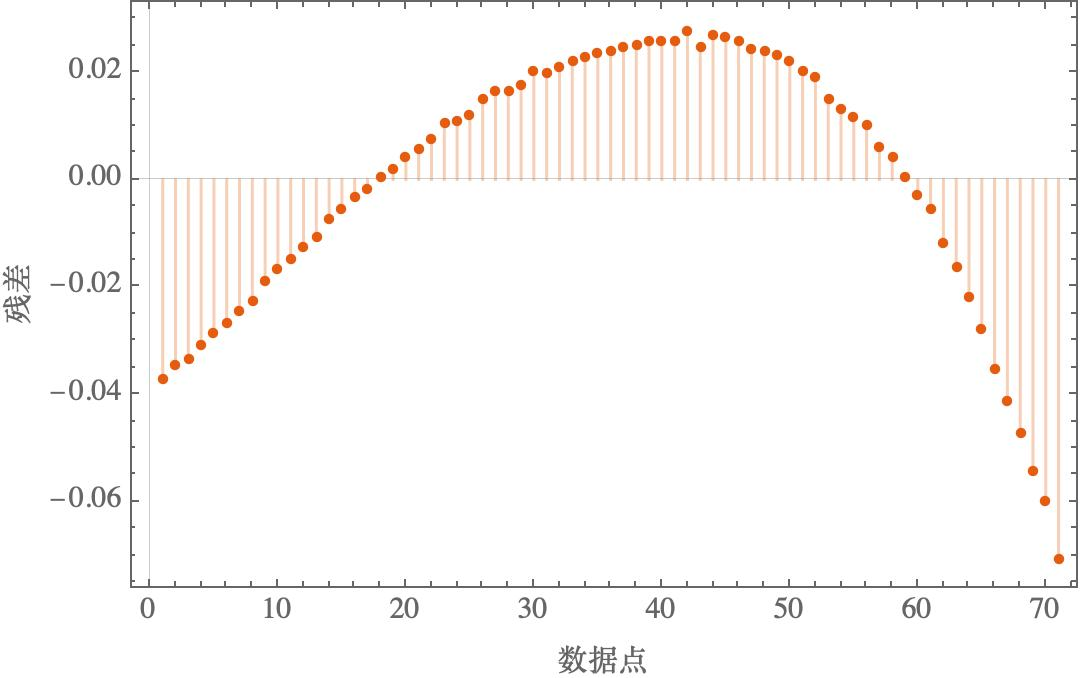
\includegraphics[scale=0.45]{residual2.jpg}
        \label{fig:first}
        \caption{组别 2 残差图}
    \end{minipage}
    \begin{minipage}[t]{0.5\linewidth}
        \centering
        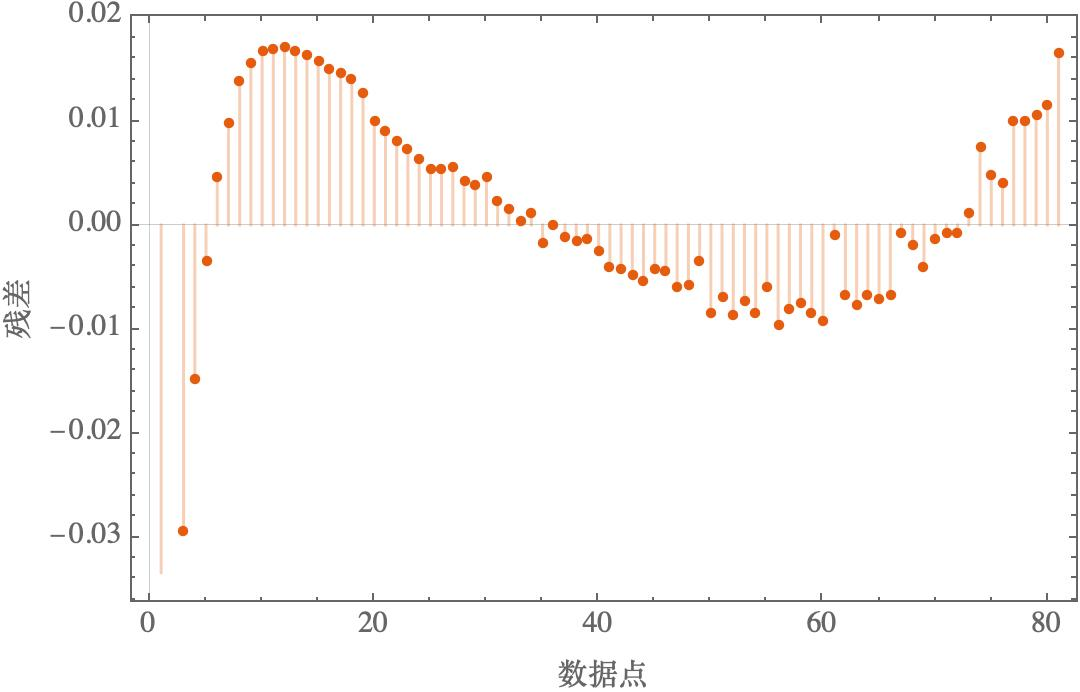
\includegraphics[scale=0.45]{residual9.jpg}
        \label{fig:second}
        \caption{组别 9 残差图}
    \end{minipage}
    \end{figure}

    很显然,残差的系统趋向违背了独立正态误差的假设,否则应当均匀地分布在水平线的两侧。所以有理由相信,蔗糖水解的副反应并不是在一定时间之后才显著出现(比如进行线性修正的图像在反应时间越过1200s后出现弯曲),而是在反应一开始就已经会有一定的影响。这一结论同样可以通过 q-q 图得到(使用Student分布并归一化),如图 3.6 所示。
    \pagebreak

\begin{figure}[ht]
    \centering
    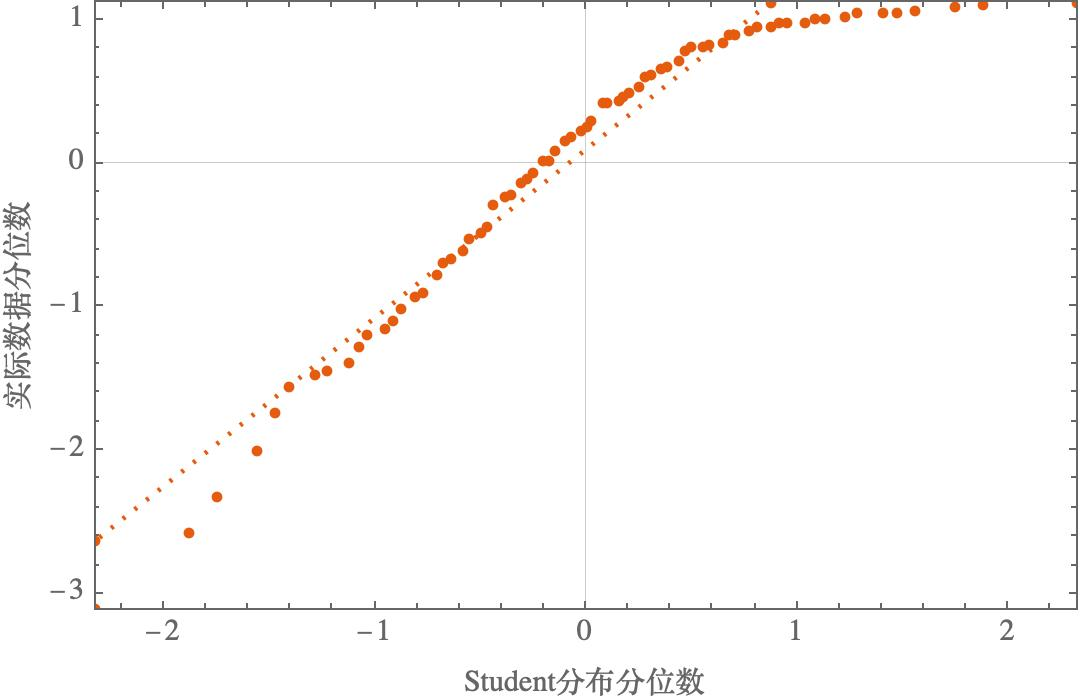
\includegraphics[width=0.6\textwidth]{qq.jpg}
    \caption{组别 2 与Student分布的q-q图}
    \label{fig:qq}
\end{figure}

显然散点图并不接近一条直线,不能认为数据集来自同一分布。

有鉴于此,对数据直接采用非线性拟合的方式,其拟合方程为
\begin{align}
    \alpha_t =e^{-kt}(\alpha_0-\alpha_{\infty} )+ \alpha _{\infty}.
\end{align}

其中将$\alpha_0$、$\alpha_{\infty}$和$k$全部视为拟合参数。该方法可以回避$\alpha_\infty$
的测定,缩短实验时间,并且能够减小实验误差。

而对数据做非线性拟合在 Mathematica 中非常容易,比如对于线性拟合中偏离较为严重的第五组实验数据的非线性拟合结果为 $-0.4349 + 1.438 \,e^{-8.732\times 10^{-4} t}$ ,图像如 3.7 所示,而残差如 3.8 所示。

\begin{figure}[!h]
    \begin{minipage}[t]{0.5\linewidth}
        \centering
        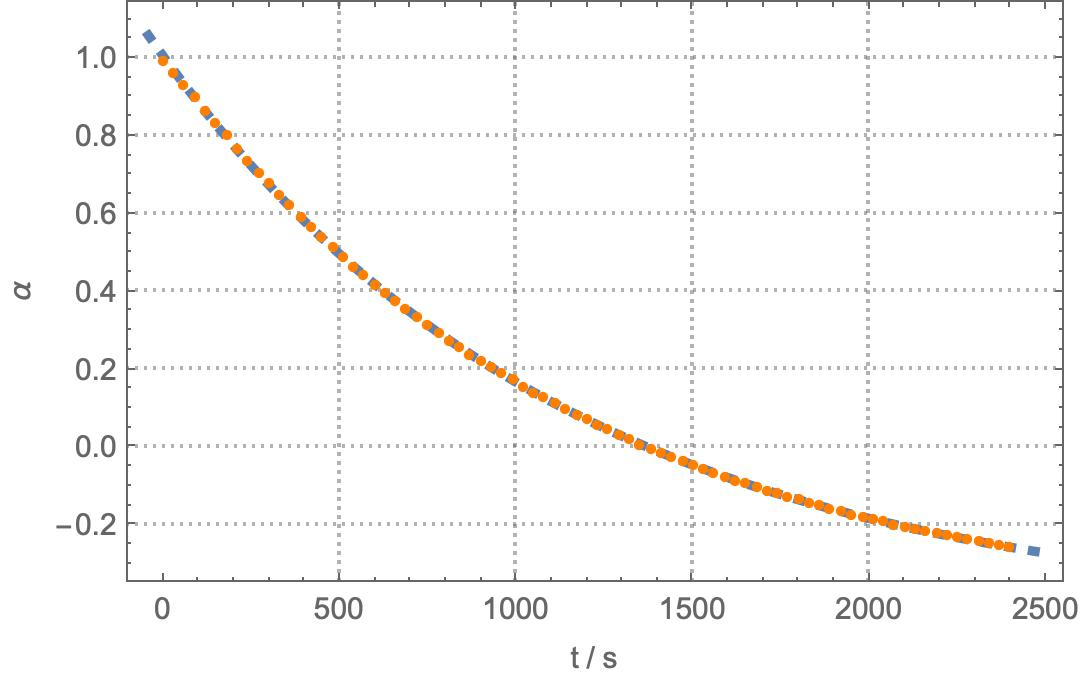
\includegraphics[scale=0.45]{nonlinear.jpg}
        \label{fig:nonlinear}
        \caption{组别 5 非线性拟合图像}
    \end{minipage}
    \begin{minipage}[t]{0.5\linewidth}
        \centering
        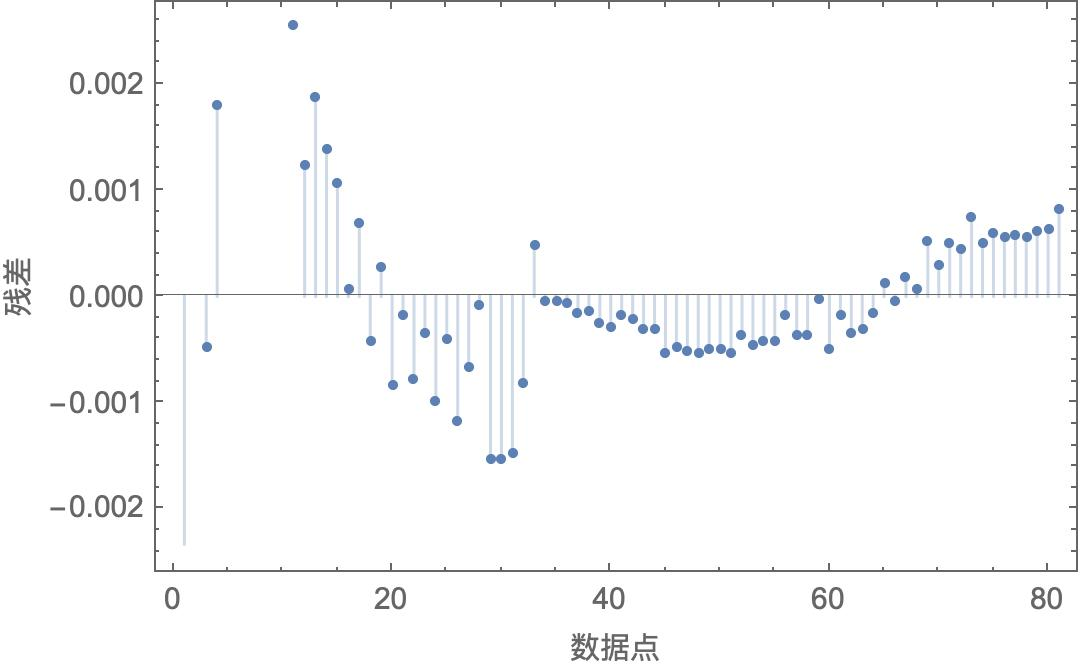
\includegraphics[scale=0.45]{renonlinear.jpg}
        \label{fig:renonlinear}
        \caption{非线性拟合残差}
    \end{minipage}
    \end{figure}

如此得到的 $k_1 = 8.732\times 10^{-4}s^{-1}$,与组别 1 所得结果再次联立,得到低浓度蔗糖、低浓度盐酸下的反应活化能 $E_a’ = 105.1 ~\mathrm{kJ\cdot mol^{-1}}$ 。与先前的结果 $E_a = 150.5 ~ \mathrm{kJ\cdot mol^{-1}} $ 比较,本方法所得结果更加接近真实值。

总之,非线性拟合的方法不再需要对 $\alpha_{\infty}$ 进行测定,提高了结果的准确性。

\subsubsection{对副反应的假设}

然而,非线性拟合的残差图仍然不服从正态假设,这指向了模型本身的问题。通过简单的分析,本实验中发生的副反应不仅严重干扰了 $\alpha_{\infty}$ 的测定,还使得使用这一参数作线性回归的过程中产生了$\alpha(t)<\alpha_{\infty}$ 和回归残差中非常明确的偏离模式,且这种偏离通过简单回避 $\alpha_{\infty}$不可消除。

所以根据实验数据分布的凹凸性,并结合在第5、6、8组观察到的 $\alpha(t)<\alpha_{\infty}, t>1500s$ 的事实,我们假设反应体系实际上存在主反应

\[
    A \mathop{\longrightarrow}^{k_1} B
\]
与副反应
\[
    B \mathop{\longrightarrow}^{k_2} C
\]
其中 $C$ 物质没有旋光性。假设副反应同样是一级反应,求解线性微分方程组
\begin{align*}
        c_1'(t)&=-k_1 c_1(t) \\
        c_2'(t)&=k_1 c_1(t)-k_2 c_2(t) \\
        c_1(0)&=c_0 ,\;\;
        c_2(0)=0
\end{align*}
得到解为
\begin{align*}
        c_1 &= c_0 e^{-k_1 t} \\
        c_2 &= -\frac{c_0 k_1 e^{-k_1 t-k_2 t}
        \left(e^{k_2 t}-e^{k_1 t}\right)}{k_1-k_2}
\end{align*}
从而总旋光度随时间的变化为
\[
    \alpha(t) = \alpha_1 c_0 e^{-k_1 t} - \alpha_2 \frac{c_0 k_1 e^{-k_1 t-k_2 t}
    \left(e^{k_2 t}-e^{k_1 t}\right)}{k_1-k_2}
\]
可以计算出函数的极值点 $t_1$ 和拐点 $t_2$ 分别是
\[
    t_1 = \frac{\ln \left(-a_1 k_1+a_2 k_1+a_1k_2\right)-\ln (a_2 k_2)}{k_1-k_2},\;\;
   t_2 = \frac{\ln \left(-a_1 k_1^2+a_2 k_1^2+a_1k_1k_2\right)-\ln (a_2 k_2^2)}{k_1-k_2}
\]
函数图像大致符合先减小,后增加、先下凸,后上凸的猜测。由于缺乏 40min 至 测量 $\alpha_{\infty}$ 时候的旋光度数据,本猜想暂时无法验证。 

\subsubsection{其他方法}
此外,还可以通过理论计算的方式得到$\alpha_\infty$的值。某一温度
下溶液的旋光度可以由下式得到
\begin{align}
    \alpha = \frac{100}{lc}[\alpha]_D^t.
\end{align}
其中$t$为测定的温度;$D$为所用光源的波长;$[\alpha]_D^t$是该条件
下的比旋光度,可以通过查阅文献资料得到;$l$是样品管的长度,在本
实验中为1 dm;c为溶液浓度,单位为 g/100 mL。

$\alpha_\infty$即为反应完全进行时溶液的旋光度。反应完全进行时,
溶液为葡萄糖和果糖的等浓度混合物。其总旋光度可以由各组分的旋光度
乘以其相应的摩尔分数得到。即
\begin{align}
    \alpha_{\text{总}}
    = x_{\text{葡}} \alpha_{\text{葡}}
    + x_{\text{果}} \alpha_{\text{果}}.
\end{align}

查阅文献得到不同温度下的比旋光度数据,就可以计算出理论的
$\alpha_\infty$值。


\section{结语}

本实验在蔗糖水解的过程中,利用旋光仪测定了糖的浓度、酸的浓度,以及
温度发生变化时体系旋光度随时间的变化。并利用 Mathematica 对数据进行线性以及非线性
拟合,计算了反应的速率常数、半衰期、初始状态的旋光度以及反应活化能
等物理化学数据。

实验结果表明,酸的浓度、反应温度都会影响速率常数,酸的浓度越大、
反应温度越高,速率常数越大,而蔗糖浓度对反应速率常数影响较小。此外
随着反应的不断进行,在高酸高温的条件下还会发生蔗糖的副反应,使
$\ln(\alpha_t-\alpha_\infty) \sim t$曲线发生弯曲。因此需要对
数据点进行适当的取舍,选用合适的数据进行线性拟合或者非线性拟合。其中数理统计方法在拟合方式上的选择有很强的辅助作用。

此外,一定的数学推导还揭示了蔗糖水解可能的副反应机理:它有可能是一个消耗生成物的一级反应,且最终产物不具有旋光性。这种反应的一个可能的实际对应,是果糖在酸性条件下被空气氧化。为了验证这一猜想,可以对反应的旋光度进行长时间的监视,并直接在旋光仪内进行升温操作,以记录下副反应对旋光度可能的影响。

最后,实验测定出反应的表观活化能在105 kJ/mol附近,这对工业上蔗糖水解制备果葡糖浆有一定的指导意义。

\newpage

\begin{center}
    \Large\bfseries{参考文献}
\end{center}
\noindent
[1] 傅献彩, 沈文霞, 姚天扬等. 物理化学(第五版). 上册[M].
高等教育出版社,2006.

\noindent
[2] 赵金和, 兰翠玲, 苏钦芳, 蒋悦夏, 陈华妮. 酸催化蔗糖水解的动力学
研究 [J]. 应用化工, 2013, 42(12): 2191-2193.

\noindent
[3] Paul M. Leininger, Martin Kilpatrick. The Inversion of
Sucrose. Journal of the American Chemical Society, 1938, 60,
12: 2891-2899.

\newpage



\begin{center}
    \LARGE\bfseries{附录~~~实验数据处理}
\end{center}
\begin{center}
    \Large\bfseries{附录I~~~实验数据处理}
\end{center}

\subsection*{I.1~~~关于 $\alpha_{\infty}$}

本实验由小组合作完成,各组实验分别的 $\alpha_{\infty}$ 由同学们提供,如表 5 所示:

\begin{longtable}{c|cccccccccc}
    \caption{各组实验的 $\alpha_{\infty}$ }\\
    \hline
    组别 & 1 & 2 & 3 & 4 & 5 & 6 & 7 & 8 & 9 & 10\\
    \hline
    $\alpha_{\infty}$ & -0.4525 & -0.4814 & -0.9046 & -0.9253 & -0.2103 & -0.4476 & -0.8321 & -0.8528& -0.3739& -0.3920 \\
    \hline
\end{longtable}

\subsection*{I.2~~~$k$的计算}

对于组1,作$\ln(\alpha_t - \alpha_\infty) \sim t$拟合,得到
拟合函数如下
\begin{align}
    \ln(\alpha_t - \alpha_\infty) = -4.438\times 10^{-4} t + 0.5910.
    \tag{I.1}
\end{align}

拟合图像如图 4.9 所示。

斜率的相反数即为速率常数,故第一组反应速率常数为
\begin{align}
    k = 4.438\times 10^{-4}~\mathrm{s^{-1}}.
    \tag{I.2}
\end{align}

\begin{figure}[!h]
    \centering
    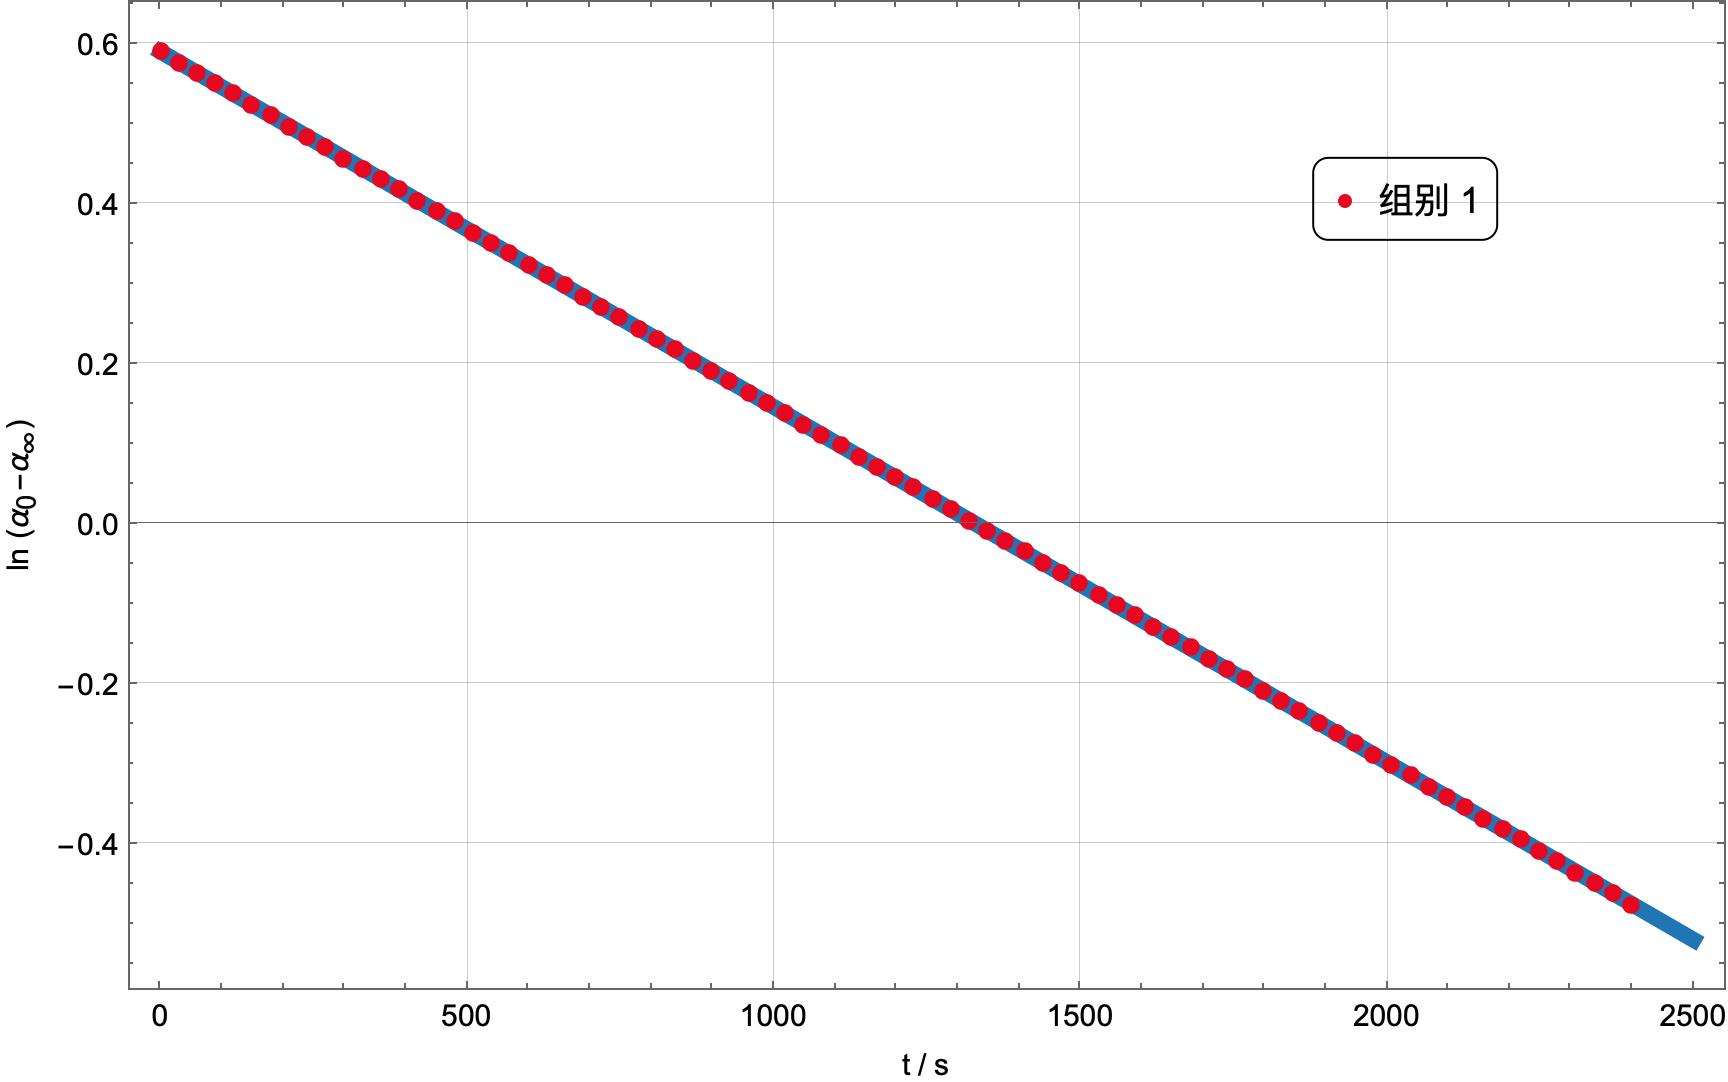
\includegraphics[scale=0.4]{first.jpg}
    \caption{第一组拟合图像}
\end{figure}

对于组2,作$\ln(\alpha_t - \alpha_\infty) \sim t$拟合,得到
拟合函数如下
\begin{align}
    \ln(\alpha_t - \alpha_\infty) = -1.488\times 10^{-3} t + 0.3713.
    \tag{I.3}
\end{align}

拟合图像如图 4.10 所示。

斜率的相反数即为速率常数,故第二组反应速率常数为
\begin{align}
    k = 1.488\times 10^{-3}~\mathrm{s^{-1}}.
    \tag{I.4}
\end{align}

\begin{figure}[!h]
    \centering
    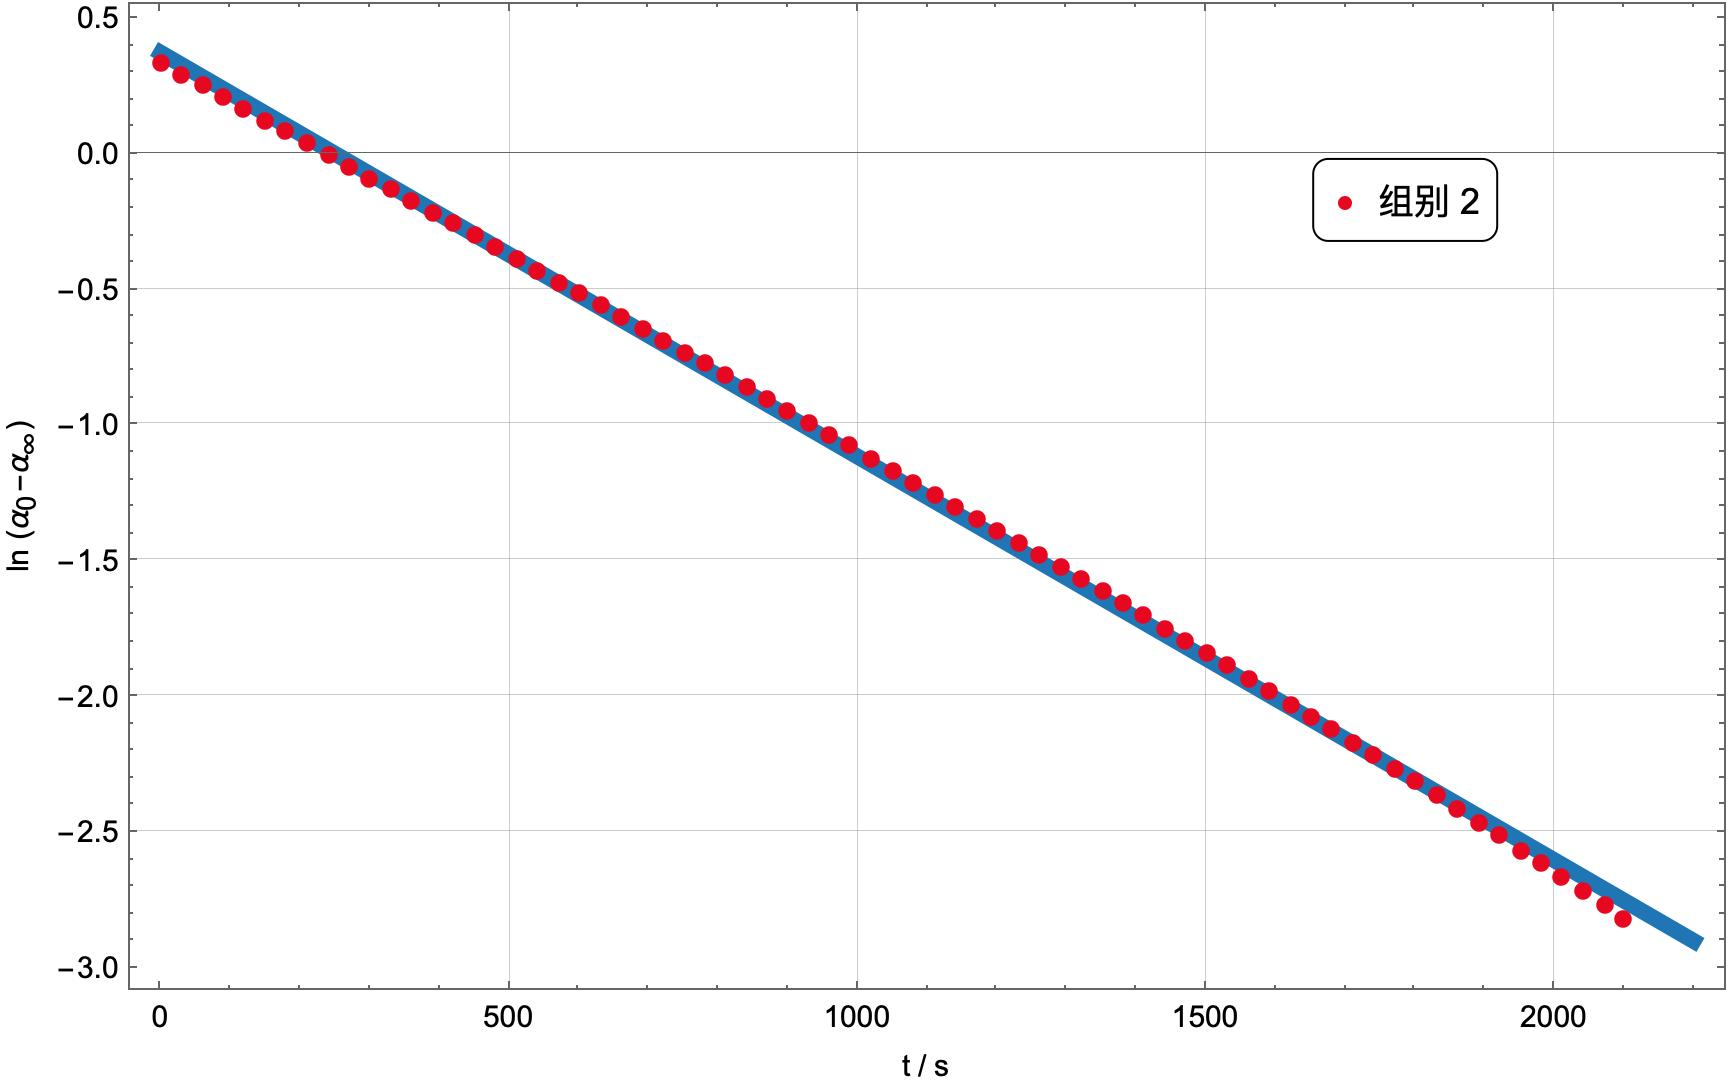
\includegraphics[scale=0.4]{second.jpg}
    \caption{第二组拟合图像}
\end{figure}

\pagebreak

\subsection*{I.3~~~$E_a$的计算}

由 Arrhenius 公式
\begin{align}
    k = A e^{-E_a/RT}.
    \tag{I.5}
\end{align}

对两边同时取对数,得到
\begin{align}
    \ln k = - \frac{E_a}{R}\frac{1}{T} + \ln A.
    \tag{I.7}
\end{align}

故作$\ln k \sim 1/T$图像即可得到反应的活化能。

若知道两个不同温度下的速率常数$k$的值,则可由积分式
\begin{align}
    \ln\frac{k_1}{k_2} = -\frac{E_a}{R}
        \left(\frac{1}{T_1} - \frac{1}{T_2}\right)
    \tag{I.8}
\end{align}
求得反应的表观活化能。

通过1、5两组实验数据可计算出,低蔗糖浓度、低氢离子浓度时蔗糖催化
水解反应的表观活化能为
\begin{align}
    E_a = 150.5~\mathrm{kJ\cdot mol^{-1}}.
    \tag{I.9}
\end{align}

通过2、6两组实验数据可计算出,低蔗糖浓度、高氢离子浓度时蔗糖催化
水解反应的表观活化能为
\begin{align}
    E_a = 107.7~\mathrm{kJ\cdot mol^{-1}}.
    \tag{I.11}
\end{align}

通过3、7两组实验数据可计算出,高蔗糖浓度、低氢离子浓度时蔗糖催化
水解反应的表观活化能为
\begin{align}
    E_a = 108.3~\mathrm{kJ\cdot mol^{-1}}.
    \tag{I.12}
\end{align}


通过4、8两组实验数据可计算出,高蔗糖浓度、高氢离子浓度时蔗糖催化
水解反应的表观活化能为
\begin{align}
    E_a = 120.3~\mathrm{kJ\cdot mol^{-1}}.
    \tag{I.10}
\end{align}

\newpage

\begin{center}
    \Large\bfseries{附录II~~~原始数据记录}
\end{center}

\begin{longtable}{cc|cc}
    \caption{30$^\circ$C 高糖高酸(每隔 30 s 记录一次)} \\
    \hline
    时间 & 旋光/$^\circ$ & 时间 & 旋光/$^\circ$ \\
    \hline
    Fri 30 Sep 2022 16:28:07 & 2.4376 & Fri 30 Sep 2022 16:46:07 & -0.1924\\
Fri 30 Sep 2022 16:28:35 & 2.3086 & Fri 30 Sep 2022 16:46:37 & -0.2232\\
Fri 30 Sep 2022 16:29:06 & 2.1789 & Fri 30 Sep 2022 16:47:07 & -0.2527\\
Fri 30 Sep 2022 16:29:36 & 2.053 & Fri 30 Sep 2022 16:47:37 & -0.2809\\
Fri 30 Sep 2022 16:30:06 & 1.9314 & Fri 30 Sep 2022 16:48:07 & -0.308\\
Fri 30 Sep 2022 16:30:36 & 1.8141 & Fri 30 Sep 2022 16:48:37 & -0.334\\
Fri 30 Sep 2022 16:31:06 & 1.701 & Fri 30 Sep 2022 16:49:06 & -0.3589\\
Fri 30 Sep 2022 16:31:36 & 1.5925 & Fri 30 Sep 2022 16:49:37 & -0.3828\\
Fri 30 Sep 2022 16:32:07 & 1.4881 & Fri 30 Sep 2022 16:50:07 & -0.4065\\
Fri 30 Sep 2022 16:32:37 & 1.388 & Fri 30 Sep 2022 16:50:37 & -0.4285\\
Fri 30 Sep 2022 16:33:07 & 1.2922 & Fri 30 Sep 2022 16:51:06 & -0.4488\\
Fri 30 Sep 2022 16:33:37 & 1.2004 & Fri 30 Sep 2022 16:51:37 & -0.4696\\
Fri 30 Sep 2022 16:34:07 & 1.1123 & Fri 30 Sep 2022 16:52:07 & -0.489\\
Fri 30 Sep 2022 16:34:37 & 1.0251 & Fri 30 Sep 2022 16:52:36 & -0.5063\\
Fri 30 Sep 2022 16:35:05 & 0.9495 & Fri 30 Sep 2022 16:53:07 & -0.5254\\
Fri 30 Sep 2022 16:35:36 & 0.8716 & Fri 30 Sep 2022 16:53:37 & -0.5423\\
Fri 30 Sep 2022 16:36:05 & 0.797 & Fri 30 Sep 2022 16:54:06 & -0.5577\\
Fri 30 Sep 2022 16:36:37 & 0.7209 & Fri 30 Sep 2022 16:54:36 & -0.5739\\
Fri 30 Sep 2022 16:37:05 & 0.6569 & Fri 30 Sep 2022 16:55:06 & -0.5891\\
Fri 30 Sep 2022 16:37:37 & 0.5869 & Fri 30 Sep 2022 16:55:37 & -0.604\\
Fri 30 Sep 2022 16:38:05 & 0.5282 & Fri 30 Sep 2022 16:56:05 & -0.617\\
Fri 30 Sep 2022 16:38:36 & 0.4658 & Fri 30 Sep 2022 16:56:37 & -0.6312\\
Fri 30 Sep 2022 16:39:07 & 0.4059 & Fri 30 Sep 2022 16:57:07 & -0.6439\\
Fri 30 Sep 2022 16:39:36 & 0.3523 & Fri 30 Sep 2022 16:57:36 & -0.6558\\
Fri 30 Sep 2022 16:40:07 & 0.2972 & Fri 30 Sep 2022 16:58:07 & -0.6675\\
Fri 30 Sep 2022 16:40:36 & 0.2478 & Fri 30 Sep 2022 16:58:36 & -0.6788\\
Fri 30 Sep 2022 16:41:07 & 0.1988 & Fri 30 Sep 2022 16:59:07 & -0.6896\\
Fri 30 Sep 2022 16:41:37 & 0.1518 & Fri 30 Sep 2022 16:59:36 & -0.7\\
Fri 30 Sep 2022 16:42:06 & 0.1069 & Fri 30 Sep 2022 17:00:07 & -0.71\\
Fri 30 Sep 2022 16:42:37 & 0.0638 & Fri 30 Sep 2022 17:00:36 & -0.7195\\
Fri 30 Sep 2022 16:43:06 & 0.0224 & Fri 30 Sep 2022 17:01:07 & -0.7286\\
Fri 30 Sep 2022 16:43:37 & -0.0173 & Fri 30 Sep 2022 17:01:36 & -0.7375\\
Fri 30 Sep 2022 16:44:06 & -0.0554 & Fri 30 Sep 2022 17:02:06 & -0.7459\\
Fri 30 Sep 2022 16:44:37 & -0.0918 & Fri 30 Sep 2022 17:02:37 & -0.754\\
Fri 30 Sep 2022 16:45:07 & -0.1267 & Fri 30 Sep 2022 17:03:07 & -0.7618\\
Fri 30 Sep 2022 16:45:36 & -0.1602\\
    \hline
\end{longtable}

\begin{longtable}{cc|cc}
    \caption{35$^\circ$C 高糖高酸(每隔 30 s 记录一次)} \\
    \hline
    时间 & 旋光/$^\circ$ & 时间 & 旋光/$^\circ$ \\
    \hline
    Fri 30 Sep 2022 17:46:08 & 1.5755 & Fri 30 Sep 2022 18:04:08 & -0.7576\\
Fri 30 Sep 2022 17:46:36 & 1.4162 & Fri 30 Sep 2022 18:04:37 & -0.7674\\
Fri 30 Sep 2022 17:47:06 & 1.2514 & Fri 30 Sep 2022 18:05:07 & -0.7767\\
Fri 30 Sep 2022 17:47:36 & 1.0914 & Fri 30 Sep 2022 18:05:38 & -0.7855\\
Fri 30 Sep 2022 17:48:06 & 0.9393 & Fri 30 Sep 2022 18:06:08 & -0.7934\\
Fri 30 Sep 2022 17:48:36 & 0.7966 & Fri 30 Sep 2022 18:06:37 & -0.8007\\
Fri 30 Sep 2022 17:49:06 & 0.6641 & Fri 30 Sep 2022 18:07:08 & -0.8073\\
Fri 30 Sep 2022 17:49:37 & 0.5368 & Fri 30 Sep 2022 18:07:38 & -0.8133\\
Fri 30 Sep 2022 17:50:07 & 0.4238 & Fri 30 Sep 2022 18:08:08 & -0.8189\\
Fri 30 Sep 2022 17:50:37 & 0.3189 & Fri 30 Sep 2022 18:08:36 & -0.8239\\
Fri 30 Sep 2022 17:51:08 & 0.2225 & Fri 30 Sep 2022 18:09:08 & -0.8287\\
Fri 30 Sep 2022 17:51:38 & 0.1334 & Fri 30 Sep 2022 18:09:38 & -0.8331\\
Fri 30 Sep 2022 17:52:08 & 0.0515 & Fri 30 Sep 2022 18:10:08 & -0.8373\\
Fri 30 Sep 2022 17:52:38 & -0.0237 & Fri 30 Sep 2022 18:10:37 & -0.8408\\
Fri 30 Sep 2022 17:53:08 & -0.0928 & Fri 30 Sep 2022 18:11:08 & -0.8443\\
Fri 30 Sep 2022 17:53:37 & -0.1565 & Fri 30 Sep 2022 18:11:38 & -0.8475\\
Fri 30 Sep 2022 17:54:08 & -0.2151 & Fri 30 Sep 2022 18:12:08 & -0.8503\\
Fri 30 Sep 2022 17:54:37 & -0.2687 & Fri 30 Sep 2022 18:12:38 & -0.8531\\
Fri 30 Sep 2022 17:55:08 & -0.3181 & Fri 30 Sep 2022 18:13:08 & -0.8554\\
Fri 30 Sep 2022 17:55:37 & -0.3635 & Fri 30 Sep 2022 18:13:38 & -0.8577\\
Fri 30 Sep 2022 17:56:08 & -0.4051 & Fri 30 Sep 2022 18:14:08 & -0.8598\\
Fri 30 Sep 2022 17:56:37 & -0.4435 & Fri 30 Sep 2022 18:14:38 & -0.8616\\
Fri 30 Sep 2022 17:57:08 & -0.4788 & Fri 30 Sep 2022 18:15:08 & -0.8634\\
Fri 30 Sep 2022 17:57:38 & -0.5113 & Fri 30 Sep 2022 18:15:36 & -0.865\\
Fri 30 Sep 2022 17:58:08 & -0.541 & Fri 30 Sep 2022 18:16:07 & -0.8665\\
Fri 30 Sep 2022 17:58:38 & -0.5685 & Fri 30 Sep 2022 18:16:38 & -0.8679\\
Fri 30 Sep 2022 17:59:07 & -0.5928 & Fri 30 Sep 2022 18:17:07 & -0.8691\\
Fri 30 Sep 2022 17:59:38 & -0.6167 & Fri 30 Sep 2022 18:17:37 & -0.8702\\
Fri 30 Sep 2022 18:00:07 & -0.6374 & Fri 30 Sep 2022 18:18:07 & -0.8713\\
Fri 30 Sep 2022 18:00:38 & -0.6579 & Fri 30 Sep 2022 18:18:37 & -0.8721\\
Fri 30 Sep 2022 18:01:08 & -0.6765 & Fri 30 Sep 2022 18:19:08 & -0.8732\\
Fri 30 Sep 2022 18:01:38 & -0.693 & Fri 30 Sep 2022 18:19:38 & -0.874\\
Fri 30 Sep 2022 18:02:07 & -0.7074 & Fri 30 Sep 2022 18:20:08 & -0.8748\\
Fri 30 Sep 2022 18:02:38 & -0.7219 & Fri 30 Sep 2022 18:20:37 & -0.8755\\
Fri 30 Sep 2022 18:03:07 & -0.7344 & Fri 30 Sep 2022 18:21:07 & -0.876\\
Fri 30 Sep 2022 18:03:37 & -0.7466\\
    \hline
\end{longtable}

\begin{figure}[ht]
    \centering
    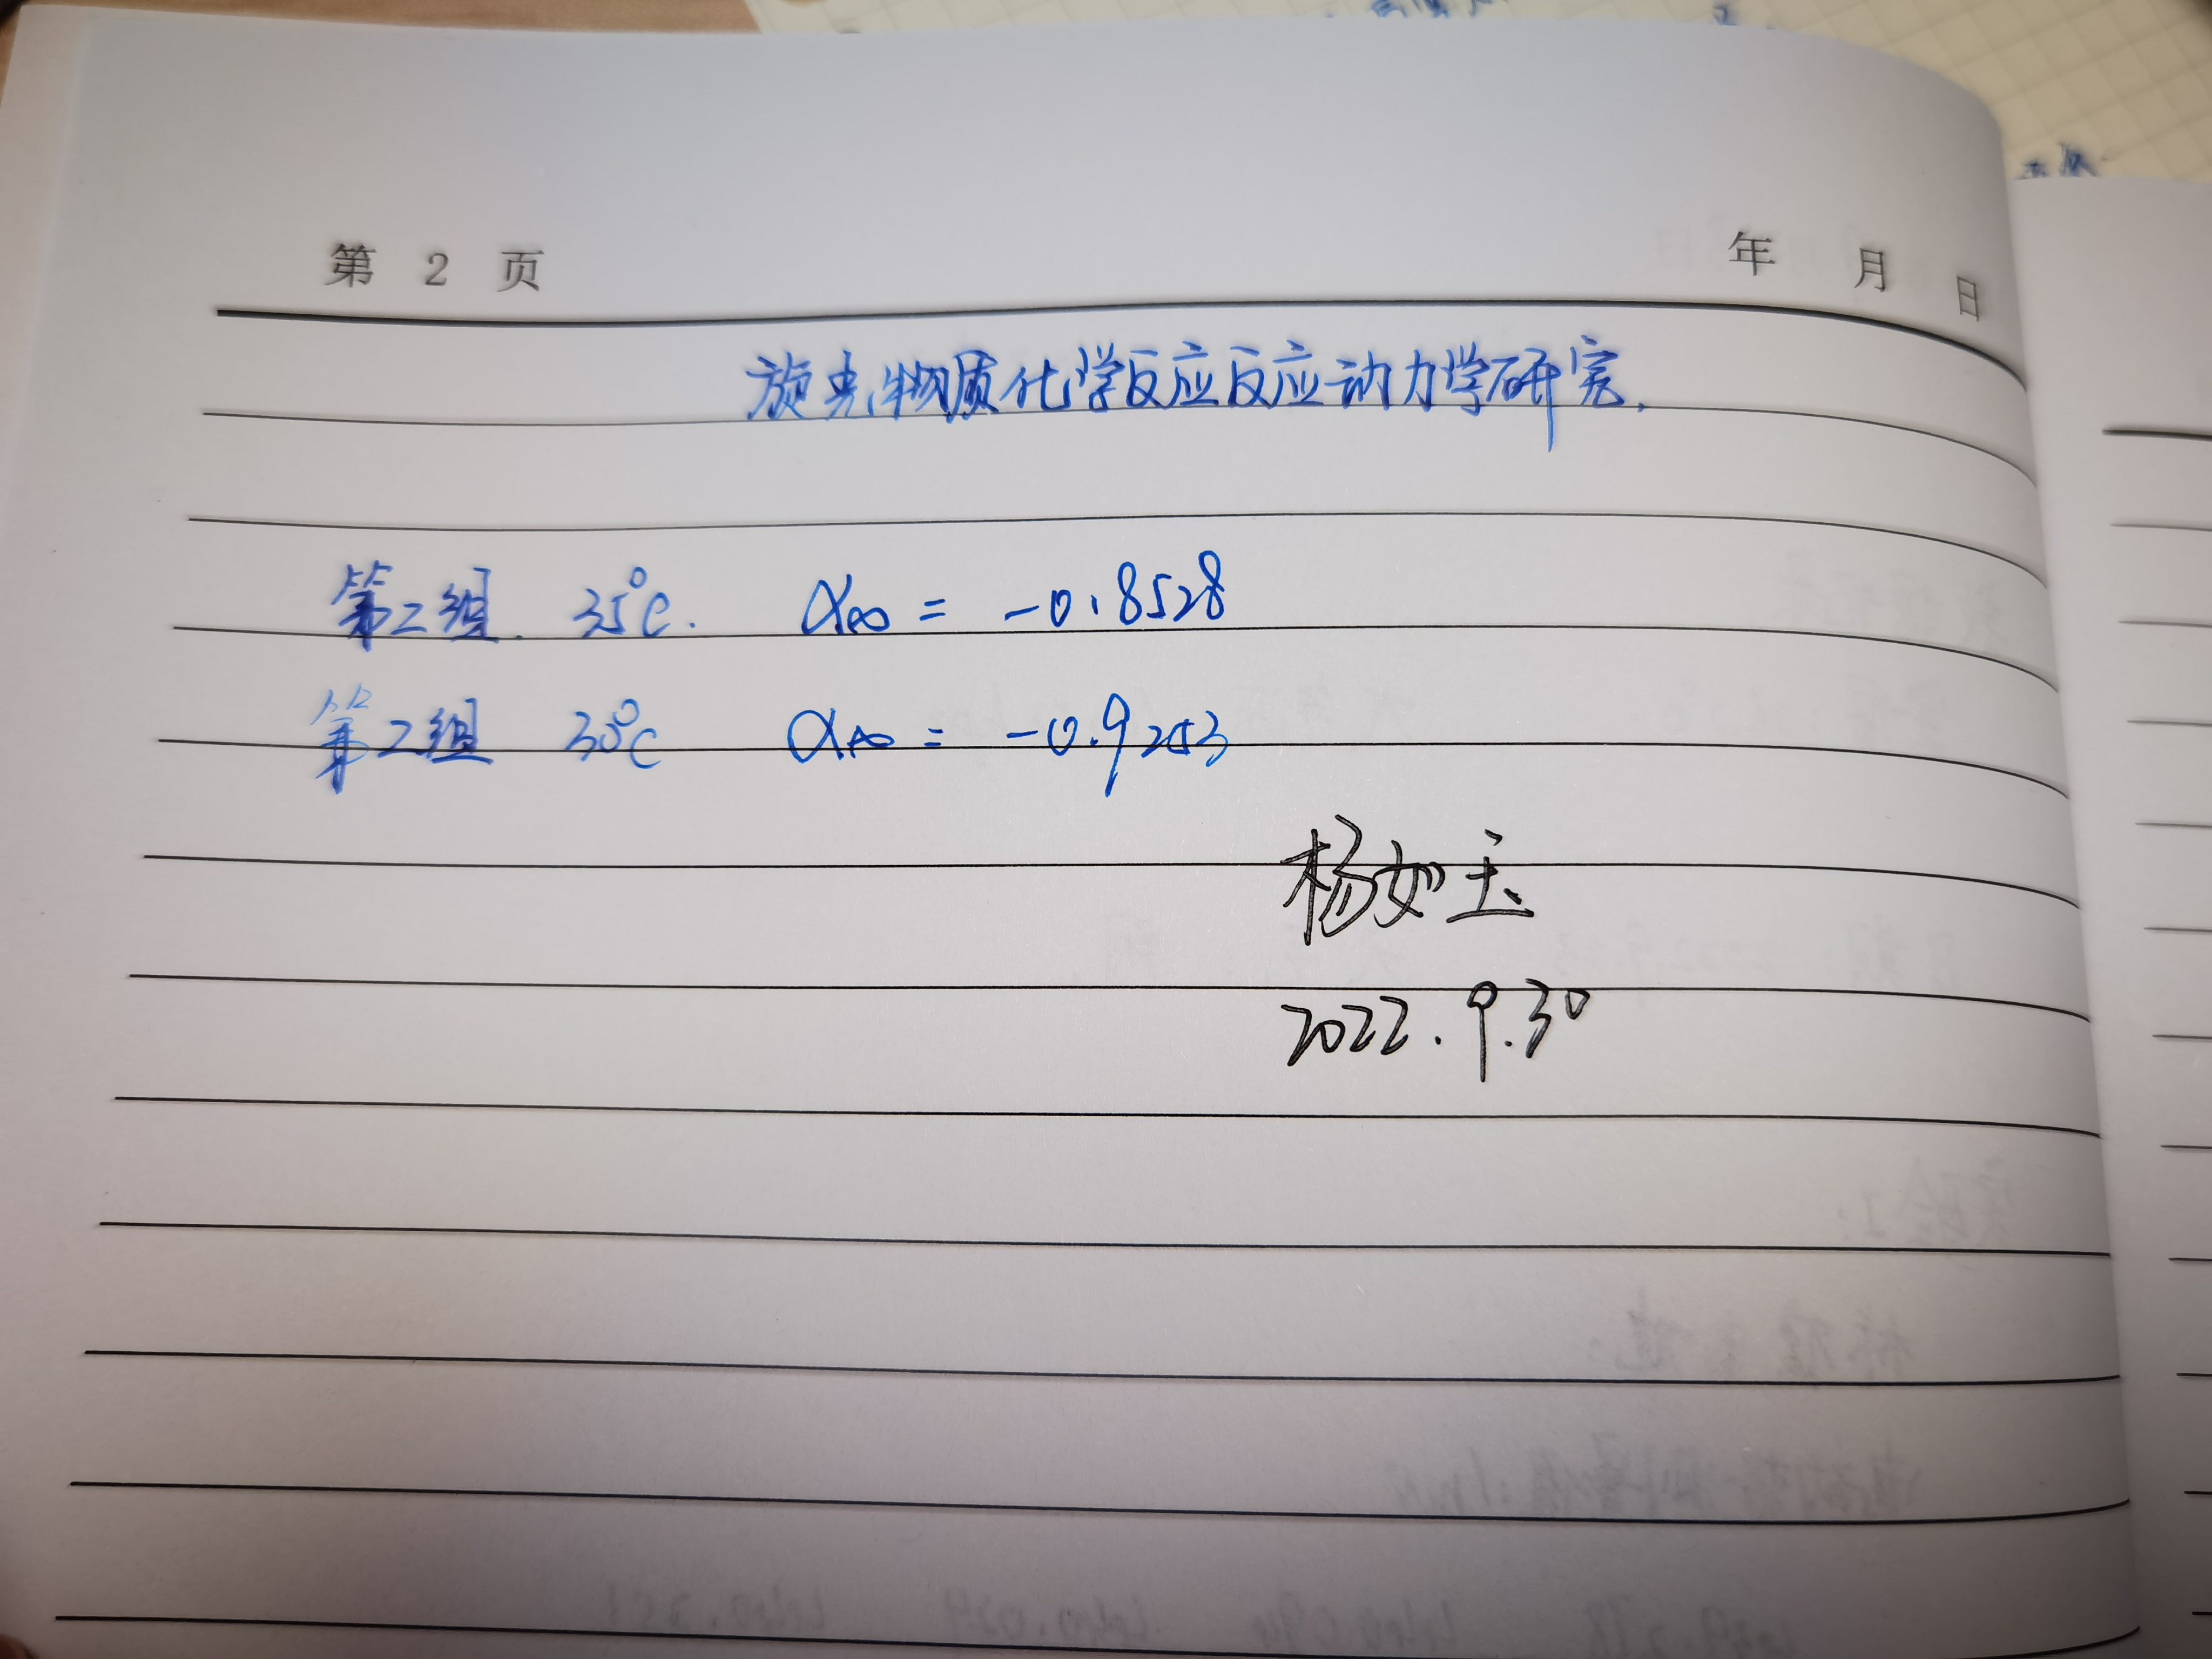
\includegraphics[width=0.6\textwidth]{原始数据.jpg}
    \caption{$\alpha_{\infty}$ 数据记录}
    \label{fig}
\end{figure}



\end{document}